\label{chap:polly}

This chapter explain the internals of  Polly - Polyhedral optimization
in llvm. The work is published in the First International workshop on PolyhedrAl Compilation
Techniques - IMPACT 2011\cite{pollypaper}.

\section{Introduction}

Today, effective polyhedral techniques exist to optimize computation intensive
programs.  Advanced data-locality optimizations are available to accelerate
sequential programs \cite{uday08pldi}. Effective methods to expose SIMD and
thread-level parallelism were developed and are used to offload calculations to
accelerators \cite{Baskaran10, Baghdadi_puttingautomatic}.  Polyhedral
techniques are even used to synthesize high-performance hardware
\cite{RISSET:2008}.

Yet, the use of programming-language-specific techniques significantly limits
their impact.  Most polyhedral tools use a basic, language specific front end
to extract relevant code regions. This often requires the source code to be in
a canonical form, disallowing any pointer arithmetic or higher level
language constructs like C++ iterators and prevents the optimization of
programs written in languages like Java or Haskell. Nevertheless, even tools
that limit themselves to a restricted subset of C may apply incorrect
transformations, as the effects of implicit type casts, integer wrapping or
aliasing are mostly ignored. To ensure correctness manual annotation
of code that is regarded safe to optimize is often required.  This prevents
automatic transformations and consequently reduces the impact of existing
tools.

In addition, significant optimization opportunities are missed by targeting a
programming language like C and subsequently passing it to a compiler. 
Effective interaction between polyhedral tools and
compiler internal optimizations are prevented. The only possible
way to pass information are source code annotations like C pragmas. As influencing
performance related decisions of the compiler is difficult, the resulting
program often suffers from poor register allocation, missed SIMDization or
similar problems.

With Polly we are developing a state-of-the-art polyhedral infrastructure for
LLVM, that supports fully automatic transformation of existing programs. Polly
detects and extracts relevant code regions without any human interaction. Since
Polly accepts LLVM-IR as input, it is programming language independent and
transparently supports constructs like C++ iterators, pointer arithmetic or
goto based loops. It is built around an advanced polyhedral library with full
support for existentially quantified variables and includes a state-of-the-art
dependency analysis. Due to a simple file interface it is easily possible to
apply transformations manually or to use an external optimizer. We use this
interface to integrate Pluto \cite{uday08pldi}, a modern data locality
optimizer and parallelizer. Thanks to integrated SIMD and OpenMP code
generation, Polly automatically takes advantage of existing and newly exposed
parallelism.

This chapter focuses on concepts of Polly which are new or little discussed in the polyhedral community.

\begin{figure}
  \label{fig:architecture}
  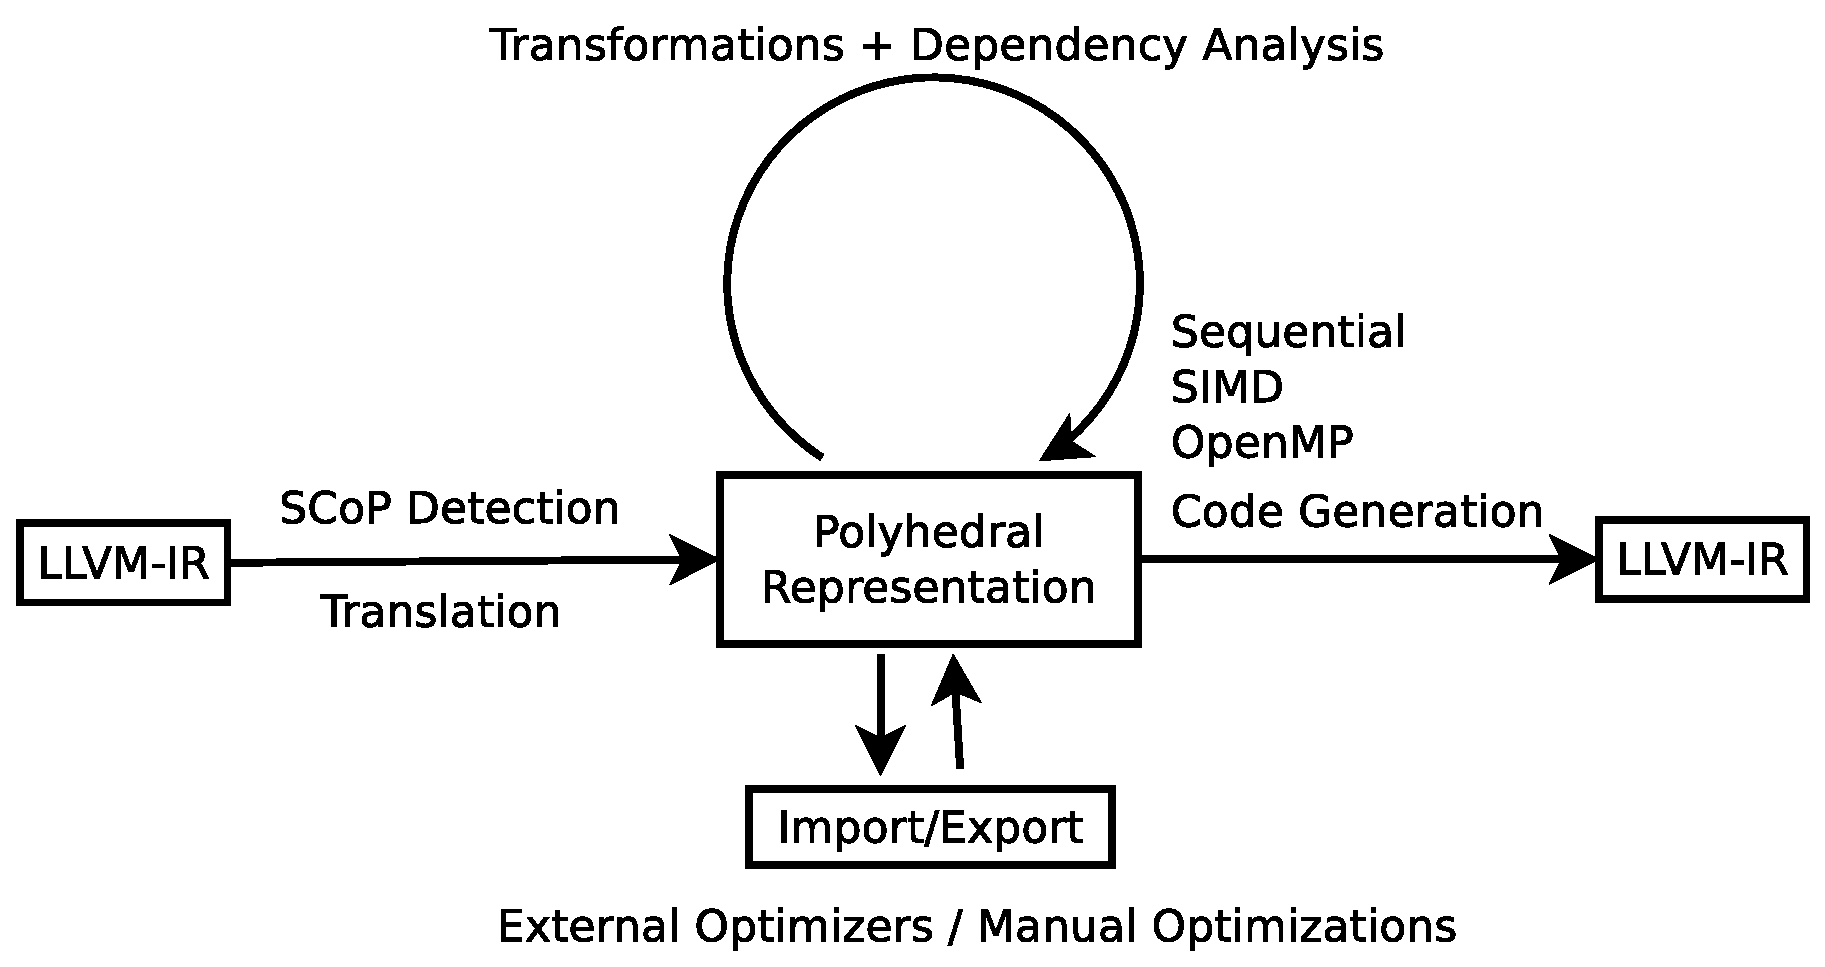
\includegraphics[width=1\textwidth]{images/architecture.eps}
  \caption{Architecture of Polly}
\end{figure}

